\documentclass[a4paper,12pt]{report}

\usepackage{alltt, fancyvrb, url}
\usepackage{graphicx}
\usepackage[utf8]{inputenc}
\usepackage{float}
\usepackage{hyperref}

\usepackage[italian]{babel}

\usepackage[italian]{cleveref}

\title{\textbf{``Programmazione ad Oggetti"}}
\author{Forti Mattia \\Marchetti Davide  \\Pagliarani Martino \\Pracucci Filippo}
\date{Giugno 2023}
\begin{document}
\maketitle

\newpage

\tableofcontents
\chapter{Analisi}
%
\section{Requisiti}
L'applicazione vuole emulare il gioco da tavolo \href{https://risiko.it/wp-content/uploads/2017/10/Regolamento-Risiko.pdf}{"Risiko"}, con qualche modifica al regolamento per rendere le partite pi\`u veloci.
La partita avverr\`a tra diversi giocatori (all'interno dello stesso calcolatore) e si dovranno seguire le regole del gioco.
Nel dettaglio si seguiranno le varie fasi della partita:
\begin{itemize}
    \item \textbf{Preparazione della partita}: distribuzione casuale degli obiettivi e dei territori e distribuzione delle armate fornite dalla dotazione iniziale di ogni giocatore .
    \item \textbf{Fase di rinforzo}: il giocatore di turno riceve un numero di armate aggiuntive in base al numero di territori in suo possesso e ai continenti conquistati. Le armate possono essere posizionate a discrezione del giocatore sui propri territori.
    \item \textbf{Fase di combattimento}: il giocatore di turno pu\`o scegliere di attaccare un territorio confinante ai propri, avviando un combattimento. In caso di vittoria l'attaccante pesca una carta e, se il territorio attaccato ha perso tutte le truppe, pu\`o scegliere quante truppe spostare dal territorio da cui ha attaccato a quello appena conquistato.
    \item \textbf{Fase di spostamento strategico}: il giocatore di turno pu\`o spostare truppe tra i propri territori, purch\'e siano adiacenti, prima di terminare il proprio turno. Una volta entrato in fase di spostamento il giocatore non potr\`a pi\`u attaccare.
\end{itemize}
Inoltre il giocatore di turno pu\`o giocare le sue carte attivando delle combinazioni prefissate, che gli permettono di ottenere truppe aggiuntive che potr\`a posizionare durante la sua fase di rinforzo al turno successivo.
%
\paragraph{Requisiti funzionali}
%
\begin{itemize}
    \item Il gioco dovr\`a permettere di gestire le varie fasi della partita, consentendo di interagire correttamente con i territori.
    \item I turni dei giocatori dovranno rispettare le fasi della partita, consentendo di compiere determinate azioni solo in caso di requisiti verificati, per esempio un giocatore non pu\`o spostare truppe da un territorio con 1 truppa ad un altro, perch\'e lascerebbe il suo territorio con 0 armate e quindi indifeso.
    \item Ad ogni turno il giocatore ricever\`a truppe aggiuntive in base ai territori conquistati.
    \item Il combattimento tra due giocatori dovr\`a essere effettuato mediante il lancio di dadi da parte di entrambi i giocatori. Il massimo di truppe attaccanti o difendenti \`e 3 e il risultato del combattimento sar\`a deciso casualmente dal lancio dei dadi.
    \item Il giocatore di turno, dopo aver conquistato un territorio, pescher\`a una carta dal mazzo delle armate. Tramite specifiche combinazioni di carte, il giocatore potr\`a ottenere delle truppe aggiuntive, che potr\`a quindi piazzare sui suoi territori al turno successivo durante la fase di rinforzo.
    \item Ogni giocatore dovr\`a arrivare al compimento del proprio obiettivo per determinare la fine della partita.
\end{itemize}
%
\paragraph{Requisiti non Funzionali}
\begin{itemize}
    \item Il gioco dovr\`a essere efficiente e reattivo ai comandi dei giocatori.
    \item I giocatori dovranno essere in grado di visualizzare il campo di gioco e i loro territori in modo intuitivo e chiaro.
    \item L'interfaccia di gioco dovr\`a essere semplice e intuitiva.
\end{itemize}
%
\section{Analisi e modello del dominio}
RisikOOP si pone l'obiettivo di simulare una partita al gioco da tavolo "Risiko" tra 3 giocatori. Il gioco prevede le interazioni tra le diverse entit\`a giocatore, le quali possiedono un'armata suddivisa sui diversi territori e un obiettivo da raggiungere per vincere la partita. I giocatori interagiscono tra loro all'interno del tabellone di gioco, il quale \`e composto da diverse entit\`a territorio che sono a loro volta raggruppate in continenti. I territori adiacenti sono collegati tra di loro permettendo il combattimento e lo spostamento di truppe. Il gioco mette a disposizione un mazzo di carte formato da tre tipologie (fanteria, cavalleria e artiglieria), da cui il giocatore pesca una carta ogniqualvolta avvenga una conquista di un territorio nemico. Lo stato del gioco \`e determinato dopo ogni fase di gioco tramite un controllo degli obiettivi di tutti i giocatori. Gli elementi costitutivi il problema sono sintetizzati in \Cref{Dominio}. Le principali difficolt\`a sono la gestione dei territori tra giocatori diversi, le azioni dei giocatori quali combattimento e spostamento e il controllo degli obiettivi di fine partita.
%
\begin{figure}[H]
\centering{}
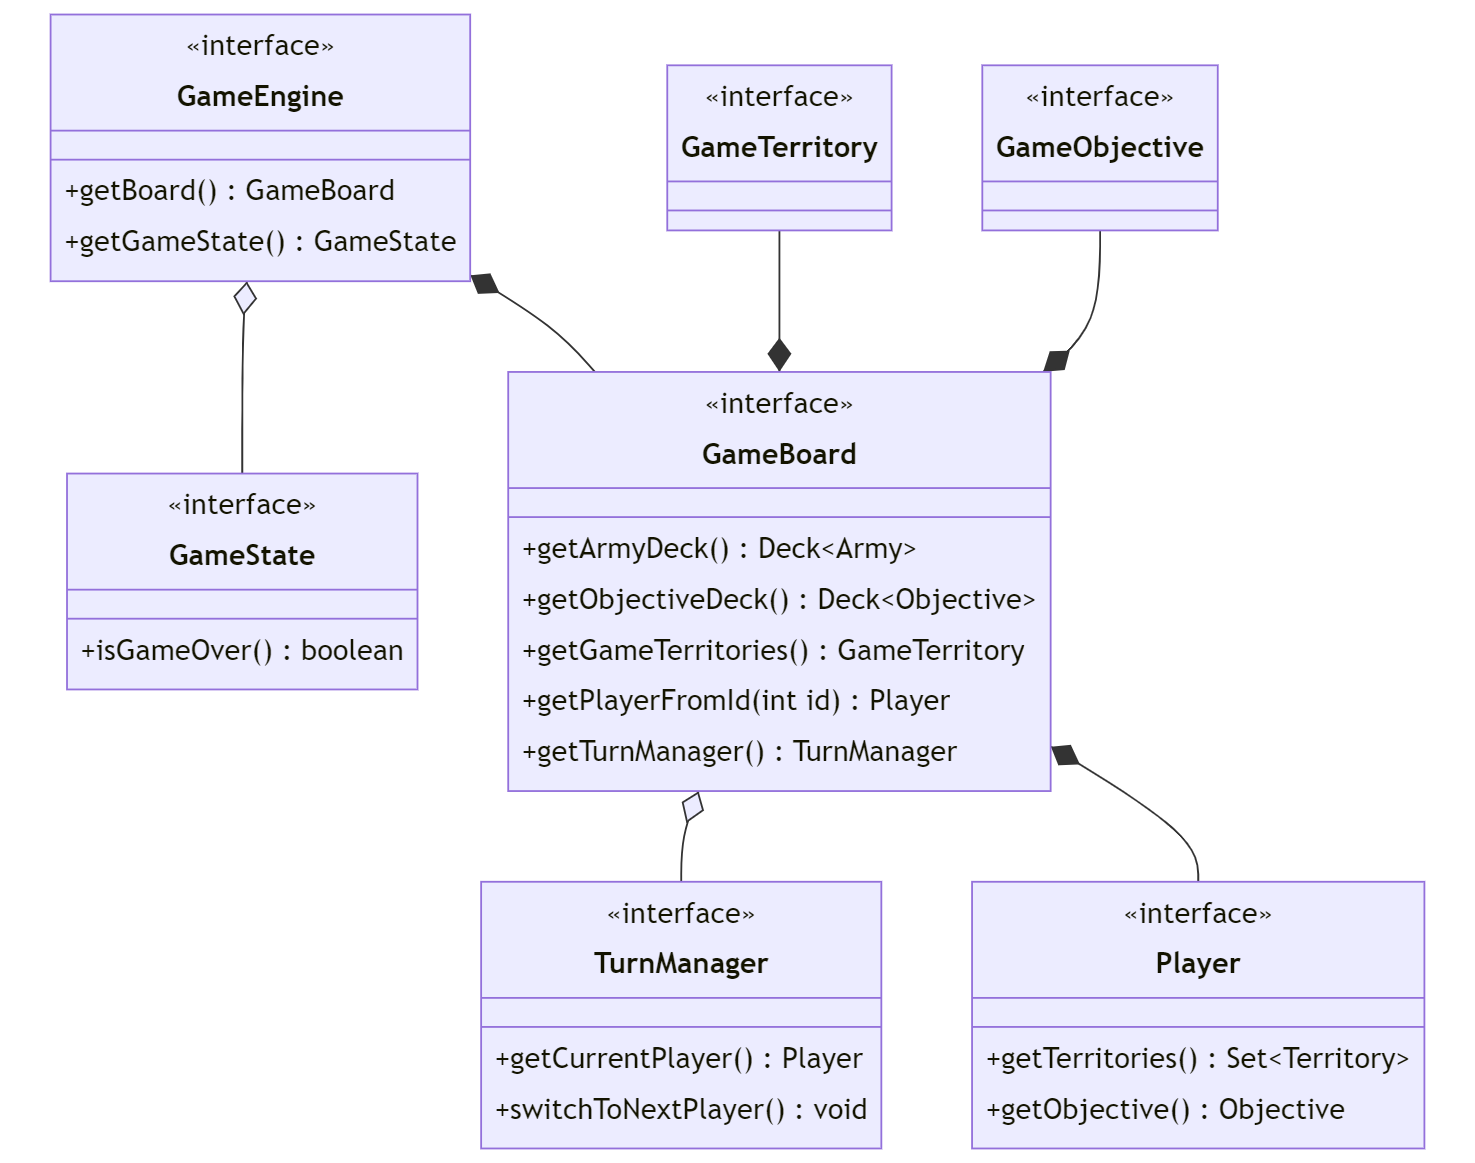
\includegraphics[width=\textwidth]{img/Model.png}
\caption{Schema UML dell'analisi del problema, con rappresentate le entit\`a principali ed i rapporti tra essi.}
\label{Dominio}
\end{figure}
%
\chapter{Design}
%
\section{Architettura}
L'architettura di RisikOOP segue il pattern architetturale MVC (Model-View-Controller) e utilizza le librerie di Java Swing per gestire l'interfaccia grafica. L'utente ha la possibilit\`a di interagire con i pulsanti dell'interfaccia grafica e, quando un pulsante viene premuto, il controller invia l'input al modello che lo processa e aggiorna i valori interni, per poi comunicare nuovamente al controller di aggiornare l'interfaccia grafica. La pressione di un pulsante determina un'azione corrispondente alla fase di gioco e al giocatore di turno. Con questa architettura possono essere aggiunti un numero arbitrario di territori, obiettivi e giocatori senza dover modificare le meccaniche di gioco. Lo stesso discorso non pu\`o essere fatto per le carte che forniscono truppe aggiuntive, in quanto si dovrebbero aggiungere nuove tipologie di carte con le relative combinazioni. In caso di aggiunta di giocatori \`e necessario aumentare il numero di carte disponibili nei vari mazzi. Di seguito viene spiegata la divisione dei ruoli seguita nel progetto per il pattern MVC:
\begin{itemize}
    \item{\textbf{Model}:} il package \textit{it.unibo.model} si occupa del modello, cio\`e della gestione di tutti i valori interni e l'esecuzione delle azioni su giocatori, territori, obiettivi e carte.
    \item{\textbf{Controller}:} il package \textit{it.unibo.controller} viene utilizzato per mettere in comunicazione il modello con le interfacce grafiche (tabellone, pannelli e finestre a comparsa) e viceversa.
    \item{\textbf{View}:} il package \textit{it.unibo.view} contiene le interfacce grafiche utilizzate. Servendosi di Java Swing, \`e stato scelto l'utilizzo di una finestra unica per separare il men\`u principale dalla schermata di gioco, cambiando all'occorrenza i pannelli contenuti al suo interno. Vengono utilizzate diverse finestre a comparsa per gli eventi di combattimento e movimento.
\end{itemize}
In \Cref{Design} si pu\`o osservare lo schema dell'architettura di RisikOOP. Viene mantenuta la modularit\`a del pattern MVC, in quanto la View pu\`o essere modificata o ampliata senza dover apportare modifiche al modello e viceversa. Questo \`e ottenibile implementando le interfacce di View gi\`a presenti che avranno le stesse funzionalit\`a delle classi create con Java Swing, evitando conflitti con il modello. Anche l'aggiunta di territori, obiettivi e giocatori non porterebbe a modifiche nella View, permettendo quindi di ampliare il gioco a proprio piacimento senza dover cambiare l'architettura iniziale.
%
\begin{figure}[H]
\centering{}
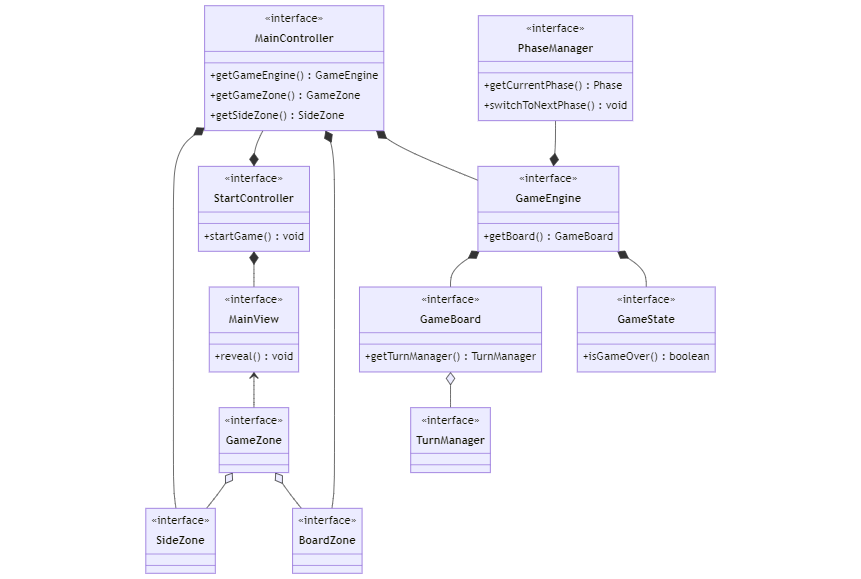
\includegraphics[width=\textwidth]{img/Detail-Model.png}
\caption{Schema UML dell'architettura di RisikOOP con tutte le parti relative al pattern MVC e le loro relazioni.}
\label{Design}
\end{figure}
%
\section{Design dettagliato}
%
\subsection{Forti Mattia}
%
\subsubsection*{Creazione del tabellone}
%
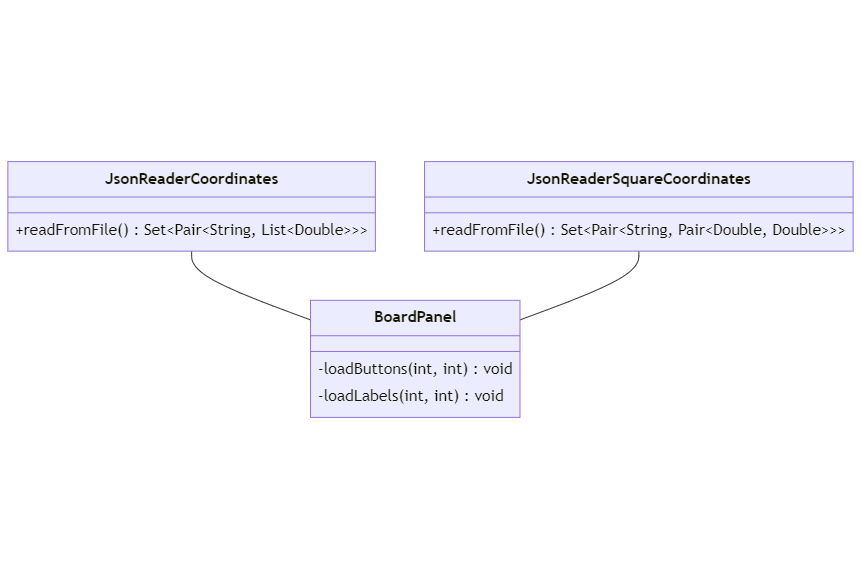
\includegraphics[width=\textwidth]{img/Board-Json.png}
%
\paragraph*{Problema} Creazione di numerosi pulsanti e etichette con posizione e dimensioni diverse all'interno di un'unica classe.
%
\paragraph*{Soluzione} Vengono usate le classi \texttt{JsonReaderCoordinates} e \linebreak \texttt{JsonReaderSquareCoordinates} per leggere tutti i dati necessari dai file \texttt{Coordinates.json} e \texttt{SquareCoordinates.json} nella cartella \textit{resources}. Questi valori vengono passati alla classe \texttt{BoardPanel} che implementa \texttt{BoardZone}, che li utilizza per creare i pulsanti dei territori e le etichette che conterranno il numero di truppe nei relativi territori.
%
\subsubsection*{Separazione dei turni dalle loro fasi}
%
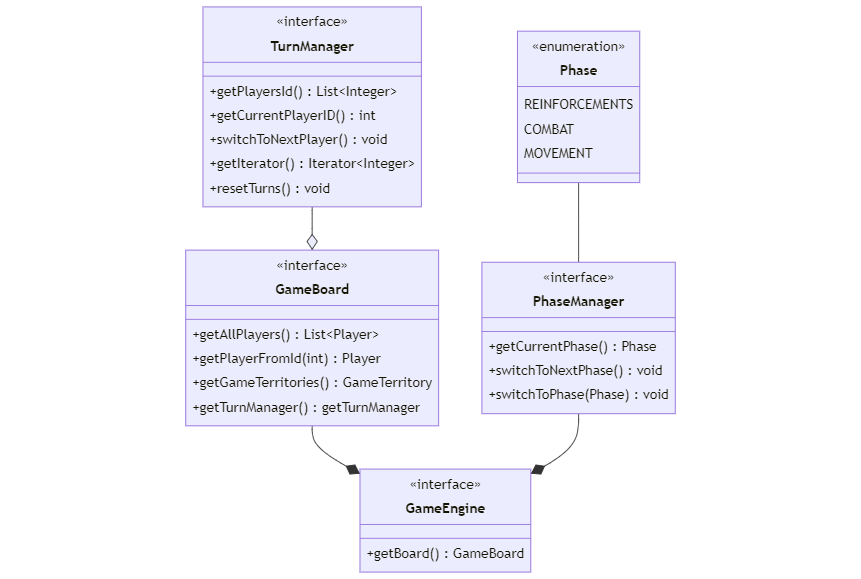
\includegraphics[width=\textwidth]{img/Turns-Phases.png}
%
\paragraph*{Problema} Ogni turno \`e suddiviso in diverse fasi nelle quali il giocatore pu\`o eseguire un'azione diversa, quindi cliccando un territorio durante le diverse fasi del turno si avranno diverse azioni, ci\`o complica la suddivisione dei compiti di gestione delle azioni eseguibili.
%
\paragraph*{Soluzione}  La classe \texttt{TurnManager} gestisce i turni dei giocatori, mentre la classe \texttt{PhaseManager} gestisce le diverse fasi di un turno. Le due classi non hanno alcun legame tra loro e lavorano indipendentemente: \texttt{TurnManager} viene usata per passare da un giocatore all'altro e viene istanziata all'interno di \texttt{GameBoard}, che a sua volta viene istanziata in \texttt{GameEngine}; \texttt{PhaseManager} viene usata per passare da una fase all'altra e viene istanziata direttamente in \texttt{GameEngine}.
%
\subsubsection*{Controllo di corretta selezione di un territorio}
%
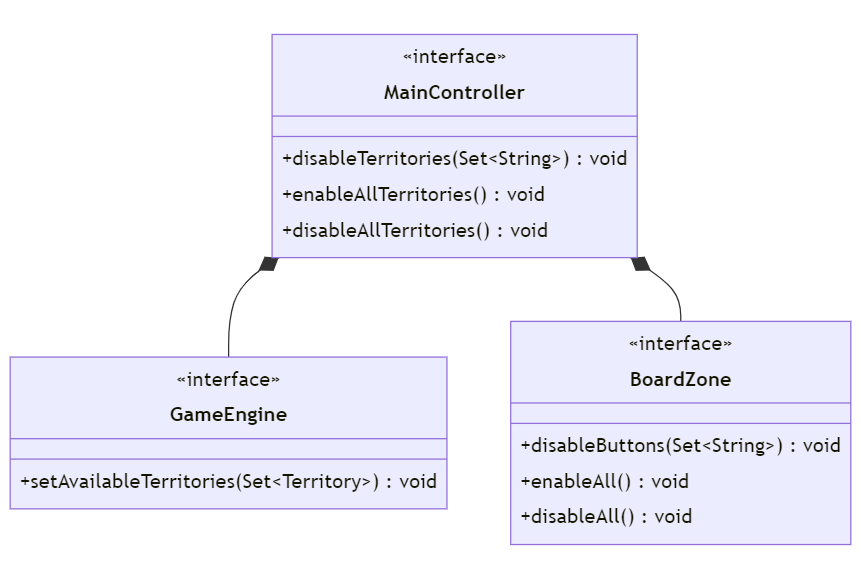
\includegraphics[width=\textwidth]{img/DisableButtons.png}
%
\paragraph*{Problema} Ogni giocatore deve essere in grado di selezionare solo i propri territori, oppure i territori nemici adiacenti in caso stia attaccando.
%
\paragraph*{Soluzione} Il metodo pi\`u efficiente per controllare se un giocatore ha cliccato un territorio valido \`e disattivare i pulsanti non validi. Ad ogni cambio di fase, il \texttt{GameEngine} identifica i territori con cui il giocatore pu\`o interagire e comunica al \texttt{MainController} di aggiornare la View, disabilitando i pulsanti non validi per la selezione. In questo modo viene eliminata la possibilit\`a di cliccare un territorio non disponibile, evitando quindi di fare un controllo inutile.
%
\subsection{Marchetti Davide}
%
\subsubsection{Gestione del combattimento tra due territori}
%
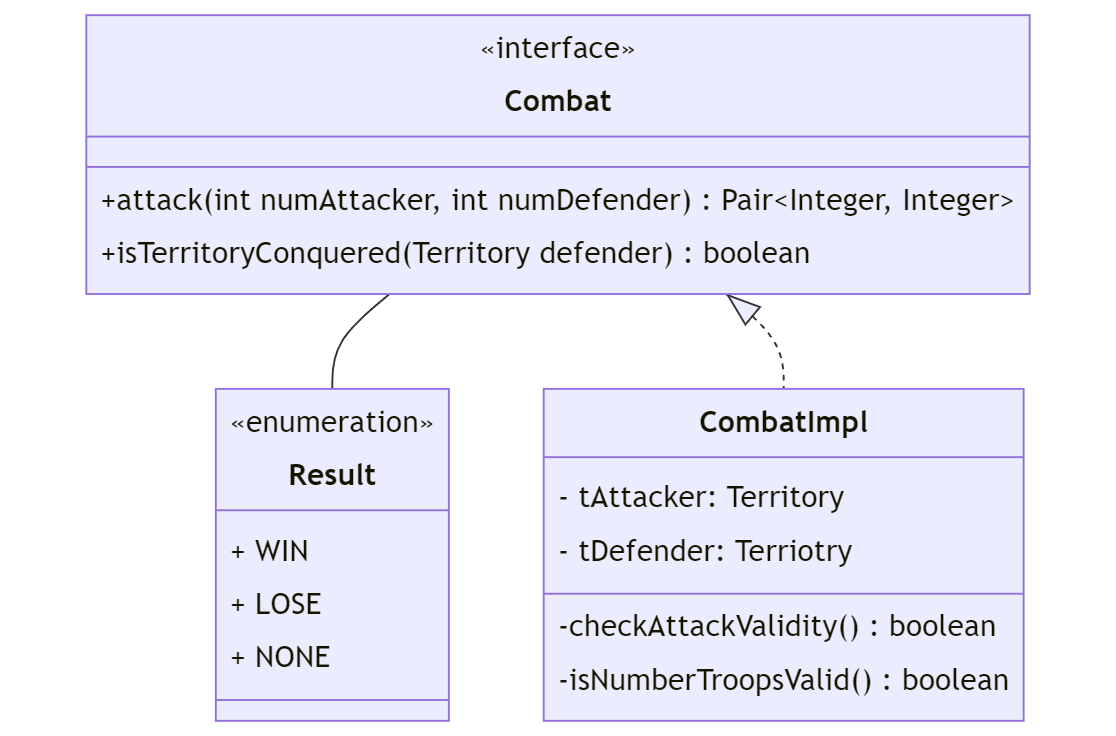
\includegraphics[width=\textwidth]{img/Combat.png}
%
\paragraph{Problema} Creazione del combattimento tra due territori presenti nella mappa di gioco utilizzando un lancio di dadi per ogni truppa selezionata dal possessore del territorio. Una volta definiti i risultati di tutti i lanci dei dadi in modo automatico, questi devono essere confrontati tra di loro per determinare il risultato del combattimento. 
%
\paragraph{Soluzione} L'interfaccia \texttt{Combat} che permette di istanziare un combattimento tra due territori, viene implementata dalla classe \texttt{CombatImpl} in cui il costruttore prende come parametri i territori interessati nel combattimento. Questa classe gestisce il combattimento seguendo dei vincoli definiti all'interno dell'implementazione dell'interfaccia. Il combattimento avviene confrontando il risultato dei dadi lanciati a coppie in ordine decrescente cos\`i da poter definire il numero di truppe che sono state sconfitte.
%
\subsubsection{Creazione dei giocatori}
%
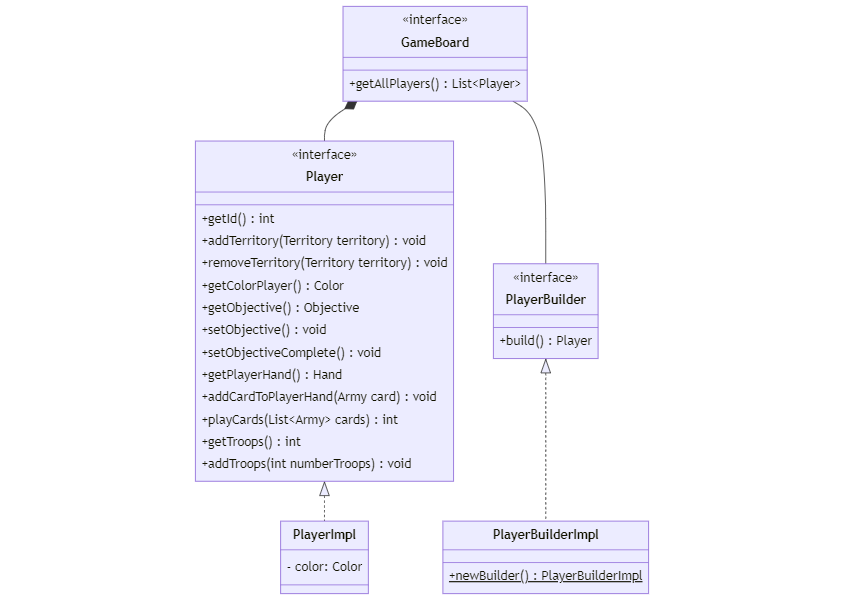
\includegraphics[width=\textwidth]{img/Player.png}
%
\paragraph{Problema} Creare un numero di giocatori definito in fase di progettazione, modellati dall'interfaccia \texttt{Player}.
%
\paragraph{Soluzione} La classe \texttt{GameBoardImpl} ha il compito di creare i giocatori della partita ed inizializzarli. Viene utilizzato il pattern creazionale \textit{Builder} con lo scopo di semplificare la creazione dei giocatori assegnando adeguati valori ai numerosi attributi dei giocatori. Viene costruito un oggetto \texttt{Player} mediante la classe \texttt{PlayerBuilderImpl}, accedendo staticamente al metodo \textit{newBuilder} e garantendo la coerenza nell'inizializzazione dell'oggetto da costruire.
%
\subsubsection{Collegamento delle varie entit\`a}
%
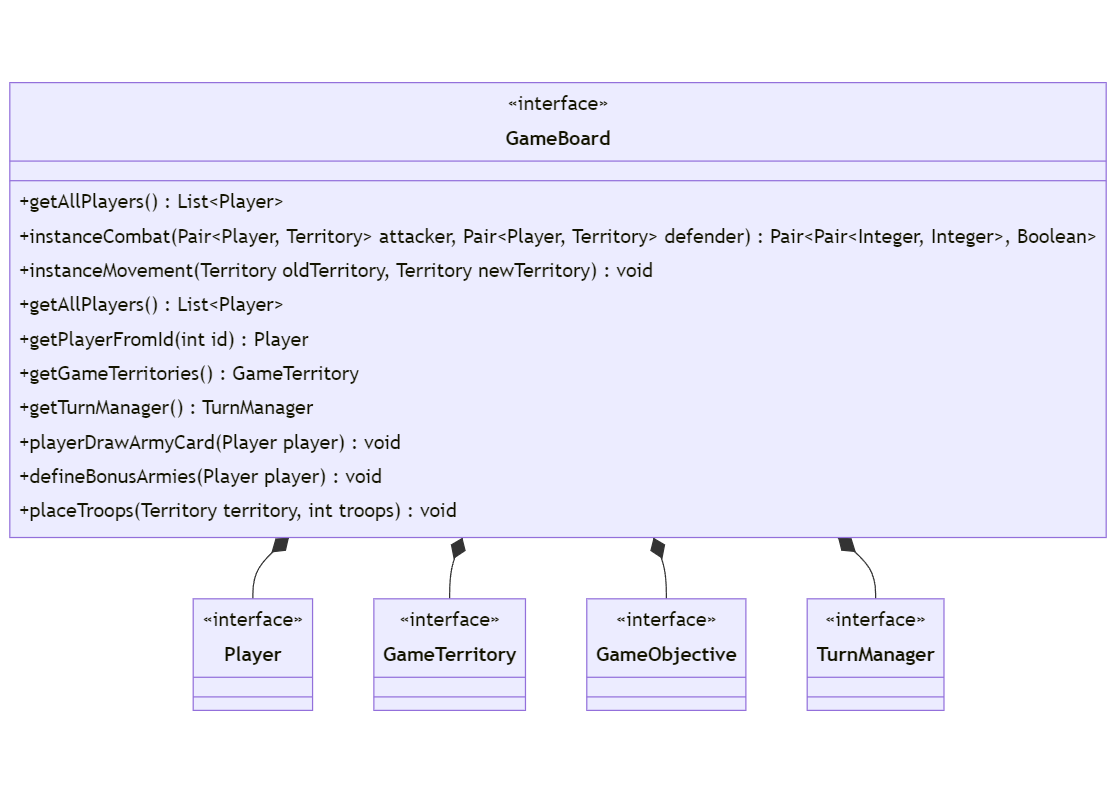
\includegraphics[width=\textwidth]{img/Board.png}
%
\paragraph{Problema} Mettere in comunicazione le varie entit\`a con il resto del modello.
%
\paragraph{Soluzione} Per mettere in comunicazione le entit\`a si fa uso dell'interfaccia \texttt{GameBoard}. Quest'ultima ha il compito di istanziare tutti gli oggetti necessari al corretto funzionamento dell'applicazione, fornendo dei meccanismi per accedervi. Inoltre mette a disposizione dei metodi per poter interagire con le istanze degli oggetti, modificandone le propriet\`a in modo adeguato senza effettuare operazioni pericolose rischiando di violare l'incapsulamento dei dati.
%
\subsection{Pagliarani Martino}
%
\subsubsection{Creazione e lettura degli obiettivi}
%
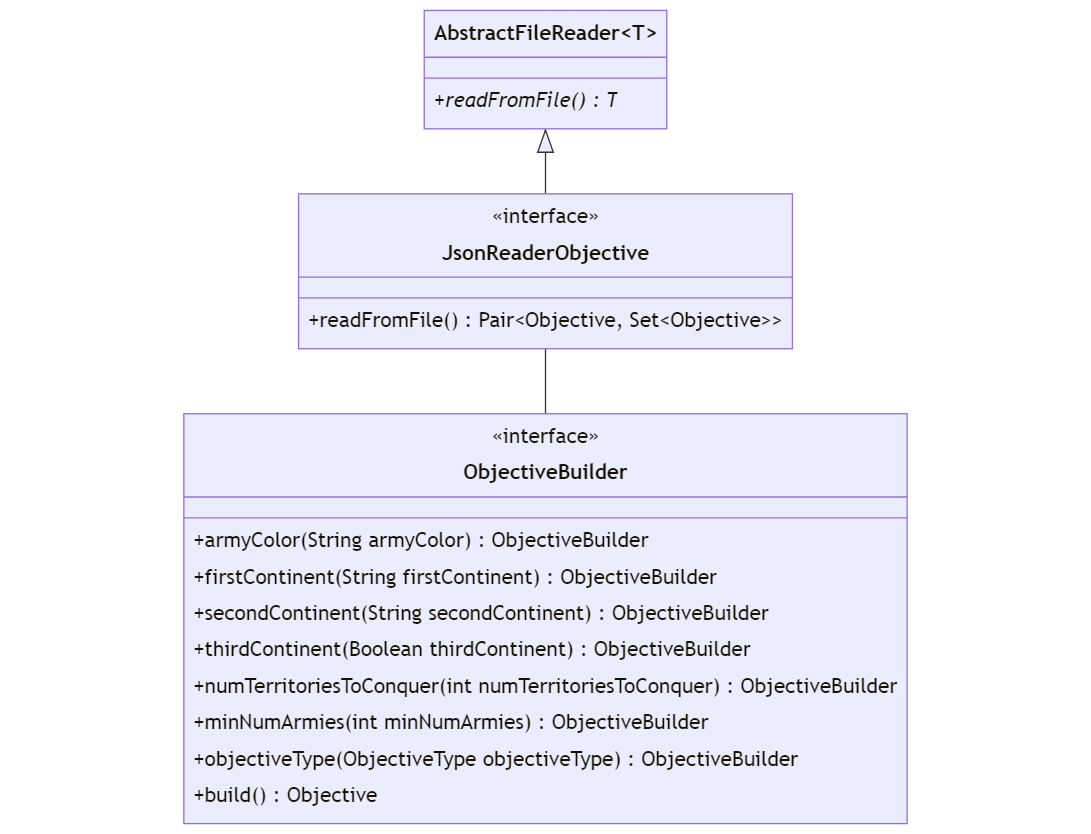
\includegraphics[width=\textwidth]{img/ReadObjective.png}
%
\paragraph*{Problema}
Creare e leggere i diversi tipi di obiettivi da un file di configurazione.
%
\paragraph*{Soluzione}
La classe \texttt{JsonReaderObjective}, che estende la classe astratta generica \texttt{AbstractFileReader}, si occupa della lettura degli obiettivi dal file di configurazione \texttt{Objectives.json}. Inoltre, viene utilizzato il pattern creazionale \textit{Builder} per assegnare i valori corretti al rispettivo obiettivo in base al suo tipo nella classe \texttt{ObjectiveBuilder}.
%
\subsubsection{Classificazione e controllo degli obiettivi}
%
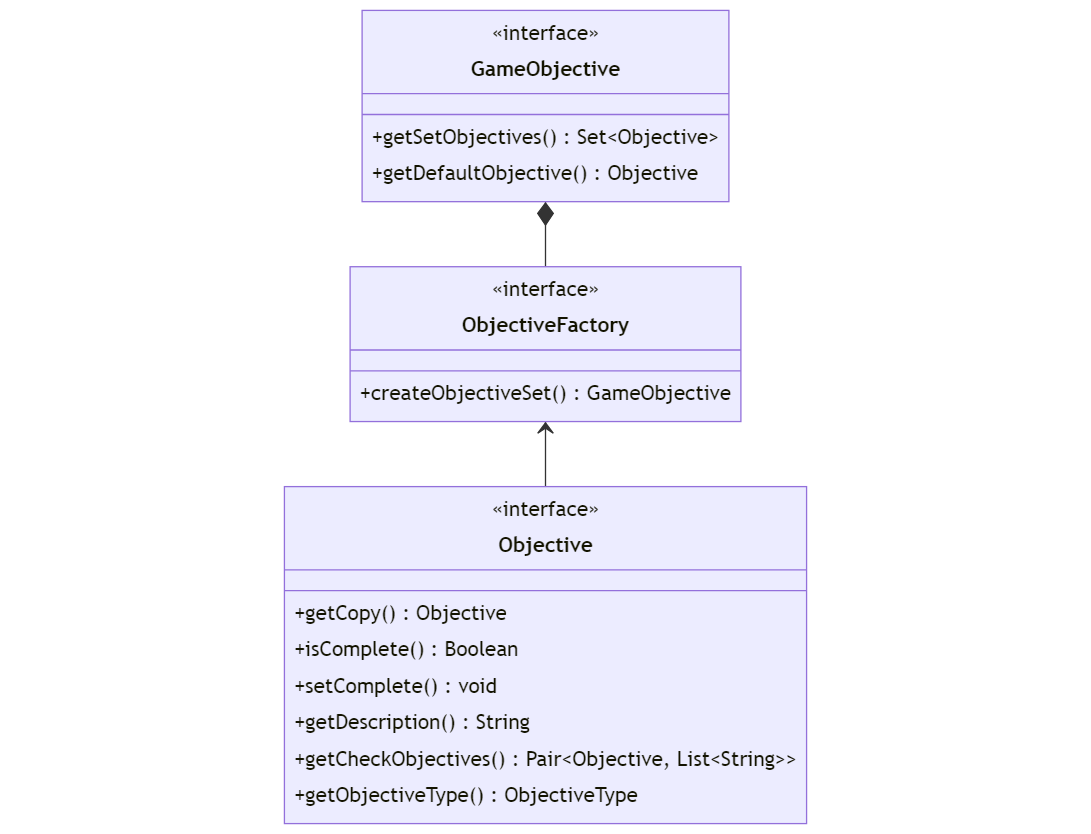
\includegraphics[width=\textwidth]{img/GameObjective.png}
%
\paragraph*{Problema}
Rappresentare i diversi tipi di obiettivi e controllarne il completamento.
%
\paragraph*{Soluzione}
Viene utilizzato il pattern creazionale \textit{Factory Method} nella classe \texttt{ObjectiveFactory} che si occupa di creare un oggetto di tipo \texttt{GameObjective} i quali metodi restituiscono l'obiettivo base e tutti gli obiettivi che la classe \texttt{GameState} controlla in base al tipo.
%
\subsection{Pracucci Filippo}
%
\subsubsection{Lettura da file}
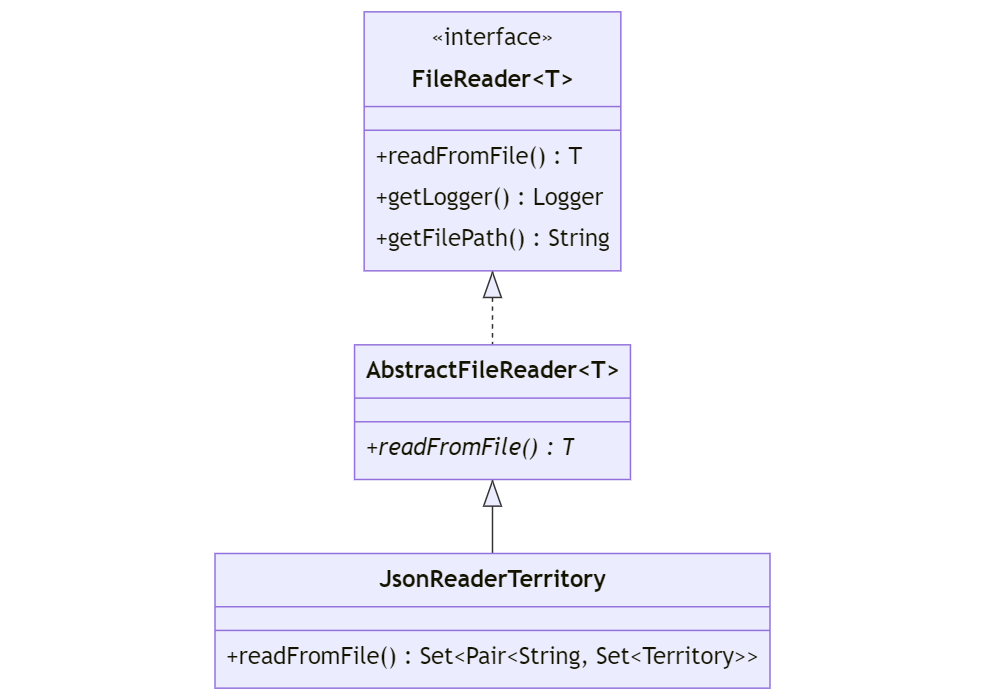
\includegraphics[width=\textwidth]{img/FileReader.png}
\paragraph*{Problema}
Lettura dei territori da un file di configurazione.
%
\paragraph*{Soluzione}
L'interfaccia \texttt{FileReader} definisce la lettura da ogni tipo di file, questa viene implementata da una classe astratta generica \linebreak\texttt{AbstractFileReader} in modo da consentire la sua estensione a diverse classi che si occupano della lettura. Nello specifico la classe \texttt{JsonReaderTerritory} la estende per leggere i territori da un file di configurazione di tipo JSON, per questo motivo viene utilizzata la libreria esterna \textit{org.json.simple}. La libreria \`e stata scelta per motivi di comodit\`a e semplicit\`a di utilizzo.
%
\subsubsection{Creazione dei territori}
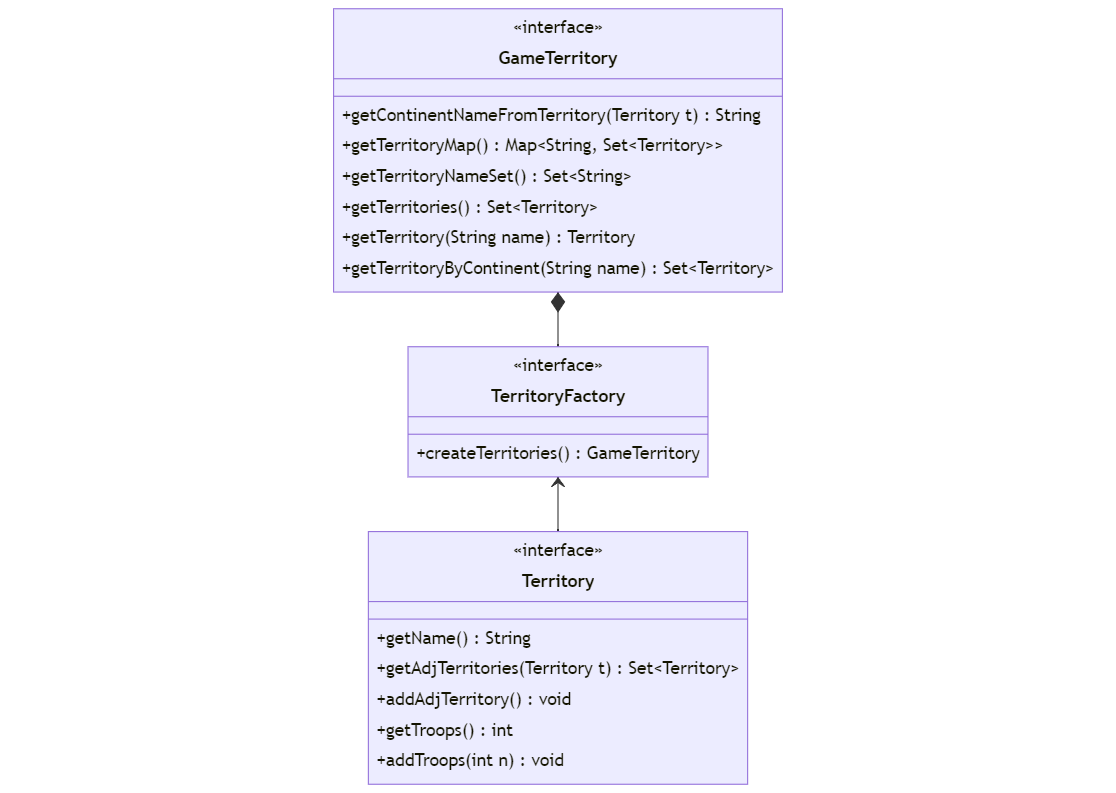
\includegraphics[width=\textwidth]{img/TerritoryFactory.png}
\paragraph*{Problema}
Creazione dei territori, suddividendoli in continenti utilizzando un file di configurazione.
%
\paragraph*{Soluzione}
Utilizzo del pattern creazionale \textit{Factory Method} che utilizza \linebreak\texttt{JsonReaderTerritory} per leggere i territori dal relativo file di configurazione. Il metodo factory \`e \textit{createTerritories()} che si occupa di creare un oggetto di tipo \texttt{GameTerritory}, cio\`e una mappa che associa ad ogni continente il corrispondente insieme di territori che lo compongono. Questa modalit\`a di creazione dei territori \`e stata scelta per facilitarne l'utilizzo all'interno dell'applicazione.
%
\chapter{Sviluppo}
%
\section{Testing automatizzato}
I test sono stati realizzati utilizzando JUnit 5 e sono:
\begin{itemize}
    \item \textbf{TestTerritory:} questa classe si occupa di controllare la correttezza della creazione dei territori. In particolare di un territorio vengono verificati nome, territori adiacenti e continente a cui appartiene.
    \item \textbf{TestObjective:} questa classe si occupa di controllare la creazione degli obiettivi di tutte le tipologie possibili: distruzione dell'armata di un avversario, conquista di continenti e conquista di un numero di territori presidiati da una minima quantit\`a di truppe.
    \item \textbf{TestCombat:} questa classe si occupa di verificare la meccanica di combattimento, quindi controlla la validit\`a del numero di attaccanti, il risultato dello scontro e la rimozione di truppe dal territorio perdente, con la possibilit\`a di conquista di un territorio.
    \item \textbf{TestMovement:} questa classe si occupa di verificare la validit\`a di uno spostamento di truppe tra due territori. Viene controllato che con lo spostamento il territorio a cui vengono tolte le truppe resti con almeno una truppa, in pi\`u i territori coinvolti nello spostamento devono essere adiacenti.
\end{itemize}
%
\section{Metodologia di lavoro}
L'architettura \`e stato il primo argomento affrontato, ragionando sulle diverse interfacce e sui nuclei del gioco, ovvero le classi principali che si occuperanno della realizzazione del pattern MVC. Il modello \`e stato suddiviso in diverse entit\`a a s\'e stanti, in modo da consentirci di effettuare un lavoro separato e riunirci solo quando necessario per discutere di eventuali problematiche o possibilit\`a di riutilizzo di varie classi. Per la realizzazione della View e del Controller invece \`e stato necessario lavorare in gruppo per collegare le diverse parti sviluppate individualmente. Abbiamo seguito un metodo di lavoro basato sul DVCS, come spiegato a lezione, creando una repository su GitHub e definendo due branch: \texttt{main} e \texttt{dev}. Sulla branch \texttt{main} abbiamo caricato solo le modifiche definitive, con classi funzionanti e senza errori di \textit{Checkstyle}, \textit{PMD} o \textit{SpotBugs}, mentre sulla branch \texttt{dev} abbiamo fatto tutte le modifiche necessarie per sistemare gli errori. Inoltre \texttt{dev} \`e stata usata come branch di prova per il funzionamento delle meccaniche di gioco.
\newline
La suddivisione dei compiti \`e presentata di seguito:
\paragraph{Forti Mattia}
%
\begin{itemize}
    \item Creazione del tabellone di gioco (package \textit{it.unibo.view.gamescreen}).
    \item Creazione della barra laterale e del pannello dei pulsanti di azione (package \textit{it.unibo.view.gamescreen}).
    \item Implementazione di un pulsante personalizzato (\texttt{CustomButton}).
    \item Logica del GameLoop (\texttt{GameEngine}), dei turni e delle fasi di gioco (package \textit{it.unibo.gameengine} e package \textit{it.unibo.model.turns}).
    \item Creazione del controller principale e sua implementazione (package \textit{it.unibo.controller.gamecontroller}).
    \item Controllo di validit\`a di spostamento delle armate tra territori (package \textit{it.unibo.model.movement}).
\end{itemize}
%
\paragraph{Marchetti Davide}
%
\begin{itemize}
    \item Creazione dei giocatori e gestione dei loro attributi (package \textit{it.unibo.model.player})
    \item Creazione e gestione di un combattimento tra territori di due giocatori (package \textit{it.unibo.model.combat})
    \item Creazione e gestione del tabellone di gioco (package \textit{it.unibo.model.board})
    \item Creazione del file \texttt{RisikoMap.jpg} contenente la mappa di gioco.
    \item Implementazione del pannello, e del rispettivo controller, che permette ai giocatori di giocare le carte (package \textit{it.unibo.view.gamescreen}), (package \textit{it.unibo.controller.playerhand}).
    \item Implementazione della view, e del rispettivo controller, per il movimento di truppe tra territori di un giocatore (package \textit{it.unibo.view.movement}), (package \textit{it.unibo.controller.movement}).
    \item Creazione e gestione del controller per avviare l'applicazione (package \textit{it.unibo.controller.gamecontroller}).
\end{itemize}
%
\paragraph{Pagliarani Martino}
%
\begin{itemize}
    \item Creazione e gestione dei mazzi di carte delle armate e degli obiettivi (package \textit{it.unibo.model.deck}, package \textit{it.unibo.model.army} e package \textit{it.unibo.model.objective}).
    \item Creazione e gestione della mano del giocatore e dei dadi (package \textit{it.unibo.model.hand} e package \textit{it.unibo.model.dice}).
    \item Creazione del file \texttt{Objectives.json} con i diversi tipi di obiettivi.
    \item Implementazione della classe \texttt{JsonReaderObjective} per la lettura da file JSON (package \textit{it.unibo.controller.reader}).
    \item Creazione e gestione della fase di preparazione della partita (package \textit{it.unibo.model.gameprep}).
    \item Controllo della condizione di fine partita (package \textit{it.unibo.gameengine.gamestate}).
    \item Creazione della finestra di combattimento (package \textit{it.unibo.view.combat}).
\end{itemize}

\paragraph{Pracucci Filippo}
%
\begin{itemize}
    \item Creazione dei territori, classificati nei diversi continenti, tramite factory (package \textit{it.unibo.model.territory}).
    \item Creazione file \texttt{Territories.json} con le definizioni di tutti i territori.
    \item Creazione dell'interfaccia \texttt{FileReader}, la sua implementazione nella classe astratta \texttt{AbstractFileReader} e relativa estensione \texttt{JsonReaderTerritory} per leggere i territori dal rispettivo file di configurazione (package \textit{it.unibo.controller.reader})
    \item Creazione \texttt{MainFrame} usato dai vari pannelli delle schermate di gioco (package \textit{it.unibo.view.gamescreen.impl})
    \item Creazione del men\`u iniziale (\texttt{MainPanel} nel package \textit{it.unibo.view.gamescreen})
    \item Pannello con le informazioni del giocatore momentaneamente in gioco (\texttt{InfoPanel} nel package \textit{it.unibo.view.gamescreen.impl})
\end{itemize}

\paragraph{Parti comuni}
%
\begin{itemize}
    \item{\texttt{GameEngine}:} unione di tutte le parti di modello sviluppate da ogni partecipante al progetto.
    \item{Interfaccia grafica:} unione del tabellone e della barra laterale all'interno della finestra di gioco.
    \item Unione dei pannelli di informazioni, carte e azioni all'interno della barra laterale
    \item{\texttt{GameBoard}:} unione di tutte le parti del modello continuativamente nel ciclo vitale dell'applicazione.
    \item Risoluzione di tutti gli errori di \textit{Checkstyle}, \textit{PMD} e \textit{SpotBugs}.
\end{itemize}
%
\section{Note di sviluppo}
%
\subsection*{Forti Mattia}
%
\subsubsection*{Utilizzo di Streams e Lambda Expressions}
%
Utilizzo di Streams e le Lambda Expressions per accorciare il codice e renderlo pi\`u intuitivo, soprattutto nelle classi che devono utilizzare le liste di territori e di giocatori. Di seguito vengono presentati alcuni esempi:
\begin{itemize}
    \item{Permalink:} \url{https://github.com/davmarc-lab/OOP22-RisikOOP/blob/8d3e7d2eda0872e91c6c40ed304b3cec7435b460/src/main/java/it/unibo/gameengine/impl/GameEngineImpl.java#L196-L198}
    \item{Permalink:} \url{https://github.com/davmarc-lab/OOP22-RisikOOP/blob/8d3e7d2eda0872e91c6c40ed304b3cec7435b460/src/main/java/it/unibo/model/movement/impl/MovementImpl.java#L39-L41}
    \item{Permalink:} \url{https://github.com/davmarc-lab/OOP22-RisikOOP/blob/8d3e7d2eda0872e91c6c40ed304b3cec7435b460/src/main/java/it/unibo/controller/gamecontroller/impl/MainControllerImpl.java#L146-L150}
\end{itemize}
%
\subsubsection*{Utilizzo di Optional}
%
Utilizzo di Optional per evitare la notazione null, cos\`i da poter inizializzare delle variabile senza valore. Di seguito un esempio:
\begin{itemize}
    \item{Permalink:} \url{https://github.com/davmarc-lab/OOP22-RisikOOP/blob/465746fdf6ee3c1d46209cce7b55c410f13fcd03/src/main/java/it/unibo/view/gamescreen/impl/BoardPanel.java#L70-L98}
\end{itemize}
%
\subsection*{Marchetti Davide}
%
\subsubsection*{Utilizzo di Streams e Lambda Expressions}
%
Utilizzo frequente per migliorare la stesura del codice e la sua leggibilit\`a. Di seguito vengono elencati alcuni esempi:
\begin{itemize}
    \item Permalink: \url{https://github.com/davmarc-lab/OOP22-RisikOOP/blob/8d3e7d2eda0872e91c6c40ed304b3cec7435b460/src/main/java/it/unibo/controller/playerhand/impl/PlayerHandControllerImpl.java#LL119C9-L121C26}
    \item Permalink: \url{https://github.com/davmarc-lab/OOP22-RisikOOP/blob/8d3e7d2eda0872e91c6c40ed304b3cec7435b460/src/main/java/it/unibo/model/board/impl/GameBoardImpl.java#LL161C9-L165C39}
    \item Permalink: \url{https://github.com/davmarc-lab/OOP22-RisikOOP/blob/8d3e7d2eda0872e91c6c40ed304b3cec7435b460/src/main/java/it/unibo/model/combat/impl/CombatImpl.java#LL171C9-L174C53}
    \item Permalink: \url{https://github.com/davmarc-lab/OOP22-RisikOOP/blob/8d3e7d2eda0872e91c6c40ed304b3cec7435b460/src/main/java/it/unibo/view/gamescreen/impl/CardPanel.java#LL138C9-L147C12}    
\end{itemize}
%
\subsection*{Pagliarani Martino}
%
\subsubsection*{Utilizzo di Streams e lambda expressions}
%
Utilizzo frequente di Streams e lambda expressions per migliorare l'efficienza e la chiarezza del codice. Alcuni esempi:
\begin{itemize}
    \item Permalink: \url{https://github.com/davmarc-lab/OOP22-RisikOOP/blob/1104a5e2bccea7b090f2a90e49414e4215243f33/src/main/java/it/unibo/model/gameprep/impl/GamePrepImpl.java#LL50C1-L68C6}
    \item Permalink: \url{https://github.com/davmarc-lab/OOP22-RisikOOP/blob/1104a5e2bccea7b090f2a90e49414e4215243f33/src/main/java/it/unibo/gameengine/impl/GameStateImpl.java#LL32C1-L36C6}
    \item Permalink: \url{https://github.com/davmarc-lab/OOP22-RisikOOP/blob/1104a5e2bccea7b090f2a90e49414e4215243f33/src/main/java/it/unibo/model/dice/impl/DiceImpl.java#LL43C1-L47C6}
\end{itemize}
%
\subsubsection*{Utilizzo di Optional}
%
Utilizzati per evitare notazioni null e definire il risultato del combattimento.
\begin{itemize}
    \item Permalink: \url{https://github.com/davmarc-lab/OOP22-RisikOOP/blob/1104a5e2bccea7b090f2a90e49414e4215243f33/src/main/java/it/unibo/controller/combat/impl/CombatControllerView.java#LL71C1-L75C6}
\end{itemize}
%
\subsection*{Pracucci Filippo}
%
\subsubsection*{Utilizzo di Streams e lambda expressions}
%
Utilizzo frequente per accorciare e rendere pi\`u intuitivo il codice, in particolare nell'uso di collezioni. Di seguito sono forniti alcuni esempi:
\begin{itemize}
    \item Permalink: \url{https://github.com/davmarc-lab/OOP22-RisikOOP/blob/1104a5e2bccea7b090f2a90e49414e4215243f33/src/main/java/it/unibo/model/territory/impl/TerritoryImpl.java#L84-L92}
    \item Permalink: \url{https://github.com/davmarc-lab/OOP22-RisikOOP/blob/1104a5e2bccea7b090f2a90e49414e4215243f33/src/main/java/it/unibo/model/territory/impl/GameTerritoryImpl.java#L33-L39}
    \item Permalink: \url{https://github.com/davmarc-lab/OOP22-RisikOOP/blob/1104a5e2bccea7b090f2a90e49414e4215243f33/src/main/java/it/unibo/model/territory/impl/GameTerritoryImpl.java#L53-L57}
\end{itemize}
%
\subsubsection*{Utilizzo di Optional}
%
Utilizzati per il caricamento dell'immagine di sfondo del men\`u principale:
\begin{itemize}
    \item Permalink: \url{https://github.com/davmarc-lab/OOP22-RisikOOP/blob/bcac1b0281f3f5b035b7cee1a16e6575492991a2/src/main/java/it/unibo/view/gamescreen/MainPanel.java#L90-L93}
\end{itemize}
%
\subsubsection*{Interfaccia e classe astratta generica}
%
Utilizzo della genericit\`a per consentire la lettura da diversi tipi di file.
\begin{itemize}
    \item Permalink: \url{https://github.com/davmarc-lab/OOP22-RisikOOP/blob/8d3e7d2eda0872e91c6c40ed304b3cec7435b460/src/main/java/it/unibo/controller/reader/impl/AbstractFileReader.java#L29}
\end{itemize}
%
\subsubsection*{Libreria esterna}
%
Utilizzo della libreria esterna \textit{org.json.simple} per consentire la lettura da file di tipo JSON.
\begin{itemize}
    \item Permalink: \url{https://github.com/davmarc-lab/OOP22-RisikOOP/blob/8d3e7d2eda0872e91c6c40ed304b3cec7435b460/src/main/java/it/unibo/controller/reader/impl/JsonReaderTerritory.java#L53-L88}
\end{itemize}

\chapter{Commenti finali}
%
\section{Autovalutazione e lavori futuri}
%
\subsection*{Forti Mattia}
%
Mi ritengo soddisfatto del lavoro svolto. \`E stato il mio primo progetto di gruppo, perci\`o non sono mancate le difficolt\`a iniziali nella decisione dell'architettura e dell'organizzazione generale del progetto, ma lavorando con gli altri, condividendo idee e opinioni, siamo riusciti a rendere la realizzazione del progetto quanto pi\`u semplice possibile. Ci\`o che pi\`u mi ha aiutato a migliorare la qualit\`a del mio codice sono stati i controlli di \textit{Checkstyle}, \textit{PMD} e \textit{SpotBugs} del \textit{Build Tool} di \textit{Gradle}, che mi hanno abituato a scrivere codice molto pi\`u "pulito" e leggibile. Lavorare sulla View mi ha interessato molto, e preferirei migliorarla, aggiungendo dettagli e animazioni, eventualmente anche con JavaFX. L'unico punto debole che mi piacerebbe risolvere in futuro con conoscenze pi\`u avanzate \`e il fatto che le partite a RisikOOP si svolgono sullo stesso calcolatore, perci\`o ogni giocatore pu\`o vedere l'obiettivo degli altri; l'ideale sarebbe renderlo un gioco online, cosicch\'e ognuno possa giocare sul proprio dispositivo senza "spiare" gli altri.
%
\subsection*{Marchetti Davide}
%
Sono molto soddisfatto del lavoro svolto insieme agli altri membri del gruppo, questo mi ha fatto capire quanto sia importante avere un confronto con altre persone durante l'analisi di un problema. Durante la realizzazione del progetto mi sono reso conto di quanto sia complesso lavorare in gruppo, in quanto richiede un'accurata organizzazione e coordinazione tra i vari membri. Nonostante ci\`o ho potuto apprezzare i numerosi vantaggi della cooperazione con gli altri partecipanti, specialmente la condivisione di opinioni diverse per raggiungere lo stesso obiettivo. Grazie ad uno strumento di controllo versione distribuito, nel nostro caso \textit{GitHub}, ci \`e risultato molto semplice riuscire a lavorare in modo efficiente. Durante l'esecuzione del progetto mi sono reso conto delle difficolt\`a nel modellare una buona architettura per un'applicazione e vorrei in futuro riuscire a migliorare in questo campo, cercando di ristrutturare questo progetto oppure dedicarmi ad un nuovo lavoro.
%
\subsection*{Pagliarani Martino}
%
Ritengo la realizzazione di questo progetto molto importante per capire il gioco di squadra all'interno di un gruppo di programmazione. Essendo il mio primo progetto, mi ha aiutato molto a mettere in pratica pi\`u su grande scala ci\`o che ho imparato in questi pochi anni di programmazione. Inoltre mi ha aiutato a capire l'importanza dell'analisi e dell'organizzazione iniziale del progetto e mi ha dato un'idea generale di come potrebbe essere il lavoro in questo ambito. I controlli forniti dal docente di \textit{Checkstyle}, \textit{PMD} e \textit{SpotBugs} sono stati molto utili a migliorare il mio stile di programmazione in quanto rendevano chiari problemi che ignoravo precedentemente ma che sono riuscito a risolvere. In futuro mi piacerebbe rivedere il progetto ampliandolo con espansioni che aggiungano modalit\`a diverse di gioco e meccaniche di gioco come potenziamenti e abilit\`a. Infine la realizzazione di questo progetto \`e stata fondamentale al percorso di studi che sto seguendo in quanto mi ha dato un'impostazione corretta e uno stile di programmazione migliore.
%
\subsection*{Pracucci Filippo}
%
La realizzazione di questo progetto mi ha fatto capire quali sono i vantaggi e le maggiori difficolt\`a nel lavoro di gruppo, in particolare lo scambio di idee e consigli \`e stato molto d'aiuto e credo mi abbia permesso di realizzare codice migliore. L'utilizzo di \textit{GitHub}, seppur in modo basilare e limitato, mi ha permesso di capire pi\`u a fondo il suo funzionamento e le sue potenzialit\`a. Il collegamento delle varie parti dell'applicazione \`e stata una delle maggiori difficolt\`a che ho riscontrato, oltre al coordinamento nel lavoro di gruppo. Lo svolgimento di un progetto di questa portata ha messo in luce la difficolt\`a nell'organizzazione di un'architettura complessa e di conseguenza la necessit\`a di ragionare a fondo sulle possibili soluzioni ad ogni problema. La stesura della relazione ha mostrato delle complicazioni, in quanto si tratta della nostra prima esperienza in tale campo, ma ci ha permesso di imparare le basi di \LaTeX{} e di organizzare innanzitutto lo scheletro dell'applicazione . In conclusione considero questa esperienza costruttiva e formante per i lavori futuri.
%
\section{Difficolt\`a incontrate e commenti per i docenti}
%
La principale difficolt\`a riscontrata \`e stata l'organizzazione dei moduli del pattern MVC, per alcune classi non eravamo sicuri del package in cui metterle e abbiamo trascorso un tempo a nostro avviso eccessivo a cercare di capire la realizzazione e il funzionamento di un Controller. Abbiamo provato a cercare delle risposte nel materiale fornito sul sito del corso e su Internet, ma abbiamo trovato soluzioni diverse allo stesso problema, creando indecisione e confusione. Riteniamo possa essere utile per gli studenti futuri ricevere una spiegazione pi\`u dettagliata sull'organizzazione dei moduli del pattern MVC o in generale fornire delle linee guida su come collegare Model e View tramite un Controller.
%
\appendix
\chapter{Guida utente}
%
All'avvio dell'applicazione l'utente verr\`a interfacciato con il men\`u principale, dove potr\`a scegliere tra i seguenti pulsanti:
%
\begin{itemize}
    \item{\texttt{PLAY}:} avvia una partita.
    \item{\texttt{QUIT}:} comparir\`a una finestra a comparsa di conferma per uscire dall'applicazione.
    \item {\texttt{RULES}:} comparir\`a una finestra a comparsa dove ci saranno scritte le regole del gioco.
\end{itemize}
%
Una volta avviata una partita ai giocatori sar\`a presentata la mappa di gioco con i vari territori su un mappamondo, mentre sulla destra troveranno una barra verticale con tre pannelli: uno per visualizzare il proprio obiettivo e il colore della propria armata, uno per giocare le carte e uno per eseguire le azioni di combattimento, spostamento e fine turno.
%
\end{document}

